\documentclass[11pt]{article}

%\newenvironment{sloppypar*}
% {\sloppy\ignorespaces}
% {\par}


\usepackage[T1]{fontenc}
\usepackage[utf8]{inputenc}
\usepackage{lmodern}
\usepackage{url}
\usepackage[english]{babel}
\usepackage{hyperref}
\usepackage{csquotes}
\usepackage[margin=1in]{geometry}
\usepackage{graphicx}
%\usepackage{tabularx}
\usepackage{lipsum}
\usepackage{booktabs}
\usepackage{multirow}
\usepackage{microtype}
\usepackage{dcolumn}
\usepackage{enumitem}
\usepackage{amsmath}

\newcommand\T{\rule{0pt}{2.6ex}}       % Top strut

\setlength{\parindent}{0em}
\setlength{\parskip}{1em}

%\hfuzz=140pt
%\newsavebox{\mybox}


\begin{document}

%\sbox{\mybox}{\hbadness=11000 \parbox{2cm}{\lipsum[1]}}


\textbf{Assignment 4 - Applied Econometrics - ECON6645}

\textbf{2022-03-17}

\textbf{Justin Desrosier}

\noindent\rule{16.51cm}{0.4pt}

\textbf{Question 1}

{
\begin{table}[!htbp]
\caption{Summary Statistics}
\centering
\def\sym#1{\ifmmode^{#1}\else\(^{#1}\)\fi}
  \begin{tabular}{rrrr}
    \hline
     Marital Status & Substance Use & Respondent Count & Median Income \\
    \hline
     Married &                   No & 28168 & 90089 \\
     &                           Yes & 1782 & 89770 \\
     &                           NA & 374 & 78637 \\
     \midrule
     Common-law &                No & 7356 & 86409 \\
     &                           Yes & 1400 & 76947 \\
     &                           NA &  63 & 69379 \\
     \midrule
     Widowed/Divorced/Separated& No & 8232 & 49192 \\
     &                           Yes & 1231 & 43321 \\
     &                           NA &  79 & 37040 \\
     \midrule
     Single &                    No & 11212 & 49758 \\
      &                          Yes & 3070 & 43645 \\
      &                          NA & 331 & 44975 \\
     \midrule
     Did not respond (NA) &      No & 172 & 61763 \\
       &                         Yes &  16 & 48953 \\
       &                         NA&6 & 56677 \\
     \hline
\end{tabular}
\end{table}
}

{
\begin{table}[!htbp]
\caption{Summary Statistics}
\centering
\def\sym#1{\ifmmode^{#1}\else\(^{#1}\)\fi}
\begin{tabular}{rrrr}
  \hline
   Highest Education & Substance Use & Respondent Count & Median Income \\
  \hline
  \T
   Less than secondary school &                   No & 5313 & 46155 \\
   &                                              Yes & 1106 & 35711 \\
   &                                              NA & 180 & 38300\\
   \midrule
   Secondary school &                             No & 11667 & 68987 \\
   &                                              Yes & 1768 & 53597 \\
   &                                              NA &  219 & 60119 \\
   \midrule
   Post-secondary diploma &                       No & 37606 & 84552 \\
   or university degree&                          Yes & 4549 & 69819 \\
   &                                              NA &  435 & 73175 \\
   \midrule
   Did not respond &                              No & 554 & 76807 \\
    &                                             Yes & 76 & 69492 \\
    &                                             NA & 19 & 85759 \\
   \hline
\end{tabular}
\end{table}
}

{
\begin{table}[!htbp]
\caption{Summary Statistics}
\centering
\def\sym#1{\ifmmode^{#1}\else\(^{#1}\)\fi}
\begin{tabular}{rrrrrr}
  \hline
 Visible Minority & Immigrant & Substance Use & Respondent Count & Median Income \\
  \hline
  \T
   No & No & No & 40004 & 81965 \\
      &    &  Yes & 5669 & 63186 \\
      &    &  NA & 577 & 64670\\
      \cmidrule(l{4em}r{1em}){2-5}
      & Yes & No & 3320 & 81449 \\
      &  & Yes & 305 & 72235\\
      &  &  NA &  62 & 70016\\
      \cmidrule(l{4em}r{1em}){2-5}
      & NA & No & 341 & 69512\\
      &  & Yes &  39 & 56625 \\
      &  & NA &   4 & 58609\\
      \midrule
   Yes & No & No & 1098 & 84489 \\
       &  & Yes & 196 & 69102 \\
       &  & NA &  24 & 65816 \\
       \cmidrule(l{4em}r{1em}){2-5}
       & Yes & No & 5732 & 67626 \\
       &  & Yes & 206 & 52942 \\
       &  & NA &  83 & 56988 \\
       \cmidrule(l{4em}r{1em}){2-5}
       & NA & No & 292 & 72326 \\
       &  & Yes &  18 & 48722 \\
       &  & NA &   5 & 86647 \\
       \midrule
    NA  & No & No & 3088 & 64462 \\
        &  & Yes & 940 & 43506 \\
        &  & NA &  60 & 61177\\
        \cmidrule(l{4em}r{1em}){2-5}
        & Yes & No & 130 & 71463 \\
        &  & Yes &   8 & 19017 \\
        &  & NA &   5 & 42347 \\
        \cmidrule(l{4em}r{1em}){2-5}
        & NA & No & 1135 & 37773 \\
        &  & Yes & 118 & 35027 \\
        &  & NA &  33 & 37334 \\
   \hline
\end{tabular}
\end{table}
}

{
\begin{table}[!htbp]
\caption{Summary Statistics}
\centering
\def\sym#1{\ifmmode^{#1}\else\(^{#1}\)\fi}
\begin{tabular}{rrrrrrr}
  \hline
  &&&&\multicolumn{3}{c}{(Age Quantile \%)}\\
 Female & Substance Use & Respondent Count & Median Income & 25th & 50th & 75th \\
  \hline
  \T
   No & No & 24209 & 82611 & 37 & 48 & 57 \\
    & Yes & 4741 & 64747 & 32 & 40 & 52 \\
    & NA & 535 & 61960 & 35 & 49 & 58 \\
  \midrule
   Yes & No & 30931 & 75092 & 36 & 47 & 56 \\
    & Yes & 2758 & 53030 & 30 & 38 & 50 \\
    & NA & 318 & 64766 & 34 & 50 & 58 \\
   \hline
\end{tabular}
\end{table}
}

\begin{figure}[!htbp]
\begin{center}
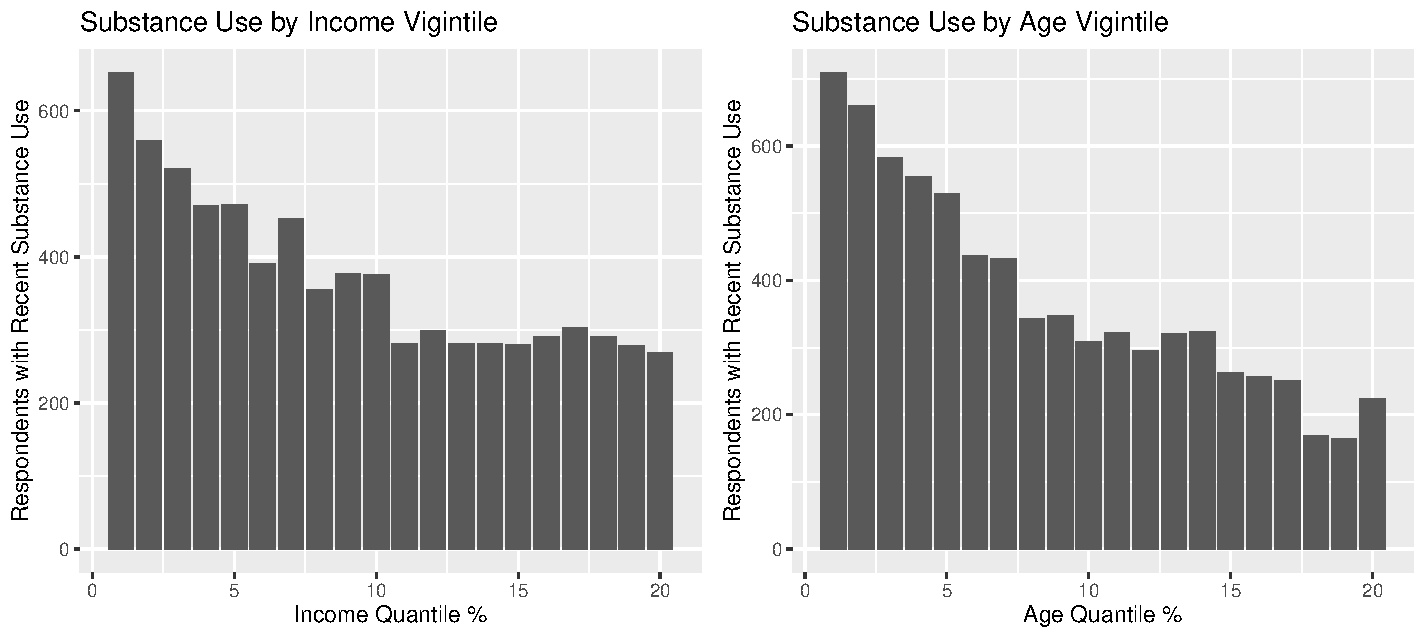
\includegraphics[height=3in,width=6in]{plots_final2}
\caption{This is a figure.}
\end{center}
\end{figure}

\vspace{10 mm}
Tables 1-4 display the summary statistics for our primary variable of interest, illict drug use in the past 12 months. The dependent variable \textit{Substance Use} is grouped against the explanatory variables income, education, marital status, immigrant and visible minority status, sex, and age. For these control variables, there will be a log trasnformation applied to income, as it is a continous variable that tends to increse exponentially. Also, as can be ascertained from Figure 1, there is a diminshing decrease in the number of respondents who have recently used illicit substances as income increases, for this reason it is also necessary to use a quadratic (squared) income control. The same does not apply to age in regard to either concern so age will be left as a continuous variable.

For the remaining control variables, they are all discrete, some are categorical while others are binary. It will be necessary to select reference categories for the non-binary variables, and leave unchanged the binary immigrant, visible minority, and sex variables. For the categorical education variable, post-secondary diploma or greater will be the reference category because a near four-fold majority of respondents are in this category. For the marital status variable, the textit{married} category contains a majority of the respondents except to a lesser extent, for this variable texit{single} will be the reference category as it the best representation of uninhibited human experience.

\begin{table}[!htbp] \centering
  \caption{Q1 Probabilistic Regression}
  \label{}
\begin{tabular}{@{\extracolsep{5pt}}lD{.}{.}{-3} D{.}{.}{-3} }
\\[-1.8ex]\hline
\hline \\[-1.8ex]
 & \multicolumn{2}{c}{\textit{Dependent variable:}} \\
\cline{2-3}
\\[-1.8ex] & \multicolumn{2}{c}{illicit} \\
\\[-1.8ex] & \multicolumn{1}{c}{\textit{OLS/LPM (1)}} & \multicolumn{1}{c}{\textit{probit (2)}} \\
\hline \\[-1.8ex]
 $log(Income)$ & -0.037^{***} & -0.186^{***} \\
  & (0.003) & (0.017) \\
\T$Income^2$ & 0.000^{***} & 0.000^{***} \\
  & (0.000) & (0.000) \\
\T \textbf{Highest Education}\\
\T\hspace{\parindent} \hspace{\parindent}\hspace{\parindent} \hspace{\parindent}$Less than Secondary School$ & 0.028^{***} & 0.124^{***} \\
  & (0.005) & (0.025) \\
\T\hspace{\parindent} \hspace{\parindent}\hspace{\parindent} \hspace{\parindent}$Secondary School$ & 0.015^{***} & 0.072^{***} \\
  & (0.003) & (0.018) \\
\T \textbf{Marital Status}\\
\T\hspace{\parindent} \hspace{\parindent}\hspace{\parindent} \hspace{\parindent}$Married$ & -0.095^{***} & -0.498^{***} \\
  & (0.004) & (0.020) \\
\T\hspace{\parindent} \hspace{\parindent}\hspace{\parindent} \hspace{\parindent}$Common\-law$ & -0.038^{***} & -0.133^{***} \\
  & (0.005) & (0.023) \\
\T\hspace{\parindent} \hspace{\parindent}\hspace{\parindent} \hspace{\parindent}$Widowed/Divorced/Separated$ & -0.027^{***} & -0.039^{*} \\
  & (0.005) & (0.024) \\
\T$Immigrant$ & -0.037^{***} & -0.268^{***} \\
  & (0.005) & (0.030) \\
\T$VisibleMinority$ & -0.051^{***} & -0.346^{***} \\
  & (0.005) & (0.034) \\
\T$Female$ & -0.078^{***} & -0.448^{***} \\
  & (0.003) & (0.015) \\
\T$Age$ & -0.004^{***} & -0.021^{***} \\
  & (0.0001) & (0.001) \\
\T Constant & 0.698^{***} & 1.732^{***} \\
  & (0.035) & (0.189) \\
  & & \\
\hline \\[-1.8ex]
Observations & \multicolumn{1}{c}{55,822} & \multicolumn{1}{c}{55,822} \\
R$^{2}$ & \multicolumn{1}{c}{0.073} &  \\
Adjusted R$^{2}$ & \multicolumn{1}{c}{0.073} &  \\
Log Likelihood &  & \multicolumn{1}{c}{-17,588.420} \\
Akaike Inf. Crit. &  & \multicolumn{1}{c}{35,200.850} \\
Residual Std. Error & \multicolumn{1}{c}{0.305 (df = 55810)} &  \\
F Statistic & \multicolumn{1}{c}{398.054$^{***}$ (df = 11; 55810)} &  \\
\hline
\hline \\[-1.8ex]
\textit{Note:}  & \multicolumn{2}{r}{$^{*}$p$<$0.1; $^{**}$p$<$0.05; $^{***}$p$<$0.01} \\
\end{tabular}
\end{table}

Table 5 (2) displays the output from a probabilistic regression of the likelihood that a responded has used an illicit drug in last 12 months on our control variables outlined above. Since the result coefficients of this model are not modified to display average marginal effects, the coefficients can be interpreted as the change in the z-score or probit index for a one unit change in the predictor \footnote[1]{https://stats.oarc.ucla.edu/r/dae/probit-regression/}. The categorical factor variables, $HighestEducation$ and $MaritalStatus$ have a slightly different interpretation. For example, having attained less than a secondary school education, versus having attained at least a post-secondary diploma (the reference group), increases teh z-score by 0.028.

\vspace{10 mm}
\textbf{Question 2}

Since our dependent variable, perceived mental health, is a multi-categorical ordinal variable, but it is not cardinal (i.e. moving between categories is not necessarily an equivalent change), we must estimate this variable's coefficients using maximum likelihood estimation.

It will also be necessary to scale (standardize) the income and age variables for this regression since they are measured in different orders of magnitude, scaling will make the coefficient results more interpretable. The categorical variables will have the same reference categories as outlined in the previous regression specification.

Table 6(2) shows the coefficients from the ordered probit regression of perceived mental health on the control variables. From the coefficients, mental health is better (from poor to fair, good, very good, excellent) with higher income although there are diminshing returns to income as can be see by the $Income^2$ coefficient. Better mental health is also associated with lower education levels, as can be seen in the categorical education coefficients with respect to the reference category, post-secondary diploma or greater level of educational attainment.

Table 6(2) also indciates that being single is associated with better mental health versus the other marital statuses. Although marriage is assocaited with at least three times less of a decline in mental health versus being single when compared to the other categories, common-law and widowed/divorced/separate. better mental health is assocaited with being an immigrant or a visible minority and not being female. Age is statistically insignificant but notably appears to have no effect.

\begin{table}[!htbp] \centering
  \caption{Ordered Probabilistic Regression}
  \label{}
\begin{tabular}{@{\extracolsep{5pt}}lD{.}{.}{-3} D{.}{.}{-3} }
\\[-1.8ex]\hline
\hline \\[-1.8ex]
 & \multicolumn{2}{c}{\textit{Dependent variable:}} \\
\cline{2-3}
\\[-1.8ex] & \multicolumn{2}{c}{Perceived Mental Health}  \\
\\[-1.8ex] & \multicolumn{1}{c}{\textit{OLS/LPM (2)}} & \multicolumn{1}{c}{\textit{ordered probit (1)}} \\
\hline \\[-1.8ex]
 $log(Income)$ & 0.209^{***} & 0.219^{***} \\
  & (0.007) & (0.008) \\
\T$Income^2$ & -0.078^{***} & -0.079^{***} \\
  & (0.006) & (0.007) \\
  \T \textbf{Highest Education}\\
\T\hspace{\parindent} \hspace{\parindent}\hspace{\parindent} \hspace{\parindent}$Less than Secondary School$ & 0.125^{***} & 0.136^{***} \\
  & (0.016) & (0.018) \\
\T\hspace{\parindent} \hspace{\parindent}\hspace{\parindent} \hspace{\parindent}$Secondary School$ & 0.187^{***} & 0.205^{***} \\
  & (0.014) & (0.016) \\
  \T \textbf{Marital Status}\\
\T\hspace{\parindent} \hspace{\parindent}\hspace{\parindent} \hspace{\parindent}$Married$ & -0.042^{***} & -0.052^{***} \\
  & (0.012) & (0.014) \\
\T\hspace{\parindent} \hspace{\parindent}\hspace{\parindent} \hspace{\parindent}$Common\-law$ & -0.187^{***} & -0.209^{***} \\
  & (0.012) & (0.014) \\
\T\hspace{\parindent} \hspace{\parindent}\hspace{\parindent} \hspace{\parindent}$Widowed/Divorced/Separated$ & -0.142^{***} & -0.162^{***} \\
  & (0.011) & (0.013) \\
\T $Immigrant$ & 0.066^{***} & 0.078^{***} \\
  & (0.014) & (0.017) \\
\T$Visible Minority$ & 0.063^{***} & 0.072^{***} \\
  & (0.016) & (0.019) \\
\T$Female$ & -0.060^{***} & -0.074^{***} \\
  & (0.008) & (0.009) \\
\T$Age$ & 0.002 & 0.004 \\
  & (0.004) & (0.005) \\
\T Constant & 2.856^{***} &  \\
  & (0.015) &  \\
  & & \\
\hline \\[-1.8ex]
Observations & \multicolumn{1}{c}{55,999} & \multicolumn{1}{c}{55,999} \\
R$^{2}$ & \multicolumn{1}{c}{0.055} &  \\
Adjusted R$^{2}$ & \multicolumn{1}{c}{0.055} &  \\
Residual Std. Error & \multicolumn{1}{c}{0.936 (df = 55987)} &  \\
F Statistic & \multicolumn{1}{c}{295.705$^{***}$ (df = 11; 55987)} &  \\
\hline
\hline \\[-1.8ex]
\textit{Note:}  & \multicolumn{2}{r}{$^{*}$p$<$0.1; $^{**}$p$<$0.05; $^{***}$p$<$0.01} \\
\end{tabular}
\end{table}

The average marginal effects of the ordered probit regression from table 6 (2) can be interpreted in the $Mean$ column as a percentage point rise (fall) in level of mental health (coeff. X 100) following a 1 standard deviation increase in the $Statistic$. For instance, a 1 standard deviation increase in income is assocaited with a decrease of 1.2 percentage points on the perceived mental health scale.

\begin{table}[!htbp] \centering
  \caption{Ordered Probabilistic Regression - Average Marginal Effects}
  \label{}
\begin{tabular}{@{\extracolsep{5pt}}lD{.}{.}{-3} D{.}{.}{-3} D{.}{.}{-3} D{.}{.}{-3} D{.}{.}{-3} }
\\[-1.8ex]\hline
\hline \\[-1.8ex]
Statistic & \multicolumn{1}{c}{Mean} & \multicolumn{1}{c}{St. Dev.} & \multicolumn{1}{c}{Min} & \multicolumn{1}{c}{Max} \\
\hline \\[-1.8ex]
\T$log(Income)$  & -0.012 & 0.008 & -0.053 & -0.004 \\
\T$Income^2$  & 0.000 & 0.000 & 0 & 0 \\
\T$Immigrant$ & -0.003 & 0.002 & -0.013 & -0.001 \\
\T$Visible Minority$  & -0.003 & 0.002 & -0.012 & -0.001 \\
\T$Female$ & 0.003 & 0.002 & 0.001 & 0.012 \\
\T$Age$  & -0.00001 & 0.00001 & -0.0001 & -0.00000 \\
\T \textbf{Highest Education}\\
\T\hspace{\parindent} \hspace{\parindent}\hspace{\parindent} \hspace{\parindent}$Less than Secondary School$ & -0.006 & 0.003 & -0.021 & -0.002 \\
\T\hspace{\parindent} \hspace{\parindent}\hspace{\parindent} \hspace{\parindent}$Secondary School$ &  -0.009 & 0.005 & -0.030 & -0.003 \\
\T \textbf{Marital Status}\\
\T\hspace{\parindent} \hspace{\parindent}\hspace{\parindent} \hspace{\parindent}$Married$ &  0.002 & 0.001 & 0.001 & 0.007 \\
\T\hspace{\parindent} \hspace{\parindent}\hspace{\parindent} \hspace{\parindent}$Common\-law$ &  0.008 & 0.004 & 0.003 & 0.030 \\
\T\hspace{\parindent} \hspace{\parindent}\hspace{\parindent} \hspace{\parindent}$Widowed/Divorced/Separated$  & 0.006 & 0.003 & 0.002 & 0.022 \\
\hline \\[-1.8ex]
\end{tabular}
\end{table}

\vspace{120mm}
\textbf{Question 3}

\begin{enumerate}[label=(\alph*)]
\item To derive a model that determines whether tobacco consumption fell as a result of the policy enactment, it is possible to use the status of similar policies in Nova Scotia as the control group in a natural experiment. The extent to which the policy effects tobacco consumption could be modelled as follows:
\vspace{-5mm}
\begin{equation*}
$TobaccoConsumption_{i,t} = {\beta}_0 + {\beta}_1T_t + {\beta}_3DiD_{i,t}+X_{i,t}{\beta}+e_i $}
\end{equation*}

\vspace{-10mm}Where $T_t$ is the difference in time from the point when the policy (T) was enacted, and the time (t) that amount of tobacco consumption is being observed. $DiD_{i,t}$ is the difference in differences coefficient that in this case estimates the difference in tobacco consumption between observations (i) (respondents) in Nova Scotia versus New Brunswick, and between the before and after time periods (t) relative to the policy change. The caveat of the model is that competing policy changes and general macroeconomic conditions could bias the results.
\item It would be possible to test the assumption of parallel trends by by viewing the difference-in-differences relationship between tobacco consumption and the explanatory variables at a point prior to the policy change. That is, change T to an earlier point in time, and view the $DiD_{i,t}$ for a before and after period within a time frame prior to the actual policy change. If there is no effect, then there is a parallel trend between the NS and NB groups and they are adequate for comparison.
\item To control for heterogenous effects between indigenous and non-indigenous peoples, we would need to define a dummy variable Z with values corresponding to whether the repondent belongs to each group.
\vspace{-5mm}
\begin{equation*}
$TobaccoConsumption_{i,t} = {\beta}_0 + {\beta}_1T_t +{\beta}_2Z_{i,t}+ {\beta}_3DiD_{i,t}+{\beta}_4(Z*T)_{i,t}+{\beta}_5INT+X_{i,t}{\beta}+e_i $}
\end{equation*}
Where, in the case of tobacco consumption following the policy change, $INT$ would be the time relative to the policy change interacted with whether the respondent was a NB or NS resident, and whether the respondent was indigenous. $INT = (Time)*(NB Resident)*(Z)$. The differnce in the coefficient $INT$ when Z=1 and Z=0 would be interpreted as the magnitude of the hetergenous effect on indigenous peoples tobacco consumption following such a policy change.

\end{enumerate}




\end{document}
